\documentclass[conference]{IEEEtran}
\usepackage[pass]{geometry}
\usepackage{amsmath,amssymb}

\usepackage{amsmath}
\usepackage{graphics}
\usepackage{caption}
\usepackage{graphicx}
\usepackage{float}
\usepackage{caption}
\usepackage{subcaption}
\restylefloat{table}
\usepackage{subcaption}
\usepackage{abstract}
\usepackage{xcolor}
\usepackage{appendix}
\usepackage{pdflscape}
\usepackage{afterpage}
\usepackage{tabularx}
\usepackage{longtable}
\usepackage{rotating}
\usepackage{fancyhdr}

\usepackage{titlesec}

\linespread{1.2}

% Make section headings bold and numbered with Arabic numerals
\renewcommand\thesection{\arabic{section}}
\titleformat{\section}
  {\bfseries\large}
  {\thesection.}
  {1em}
  {}

% Make subsection headings bold and numbered with Arabic numerals
\renewcommand\thesubsection{\thesection.\arabic{subsection}}
\titleformat{\subsection}
  {\bfseries}
  {\thesubsection.}
  {1em}
  {}

% Make subsubsection headings bold and numbered with Arabic numerals
\renewcommand\thesubsubsection{\thesubsection.\arabic{subsubsection}}
\titleformat{\subsubsection}
  {\bfseries}
  {\thesubsubsection.}
  {1em}
  {}
  
\begin{document}
 
\title{Arkis v2: Bridging the Gap Between CEX and DEX Liquidity}
\author{Proskurin Oleksandr}

\maketitle
    \begin{abstract}
Arkis v2 introduces enhanced functionalities catering to Asset Managers seeking perpetual futures trading capabilities. This iteration builds upon the foundation laid by Arkis Margin Engine v1, with a primary emphasis on elucidating perpetual futures risk analysis and the seamless integration of CeFi and DeFi components within Arkis portfolios.
Key findings: 
\begin{enumerate}
  \item The new protocol design fosters a permissionless environment, enabling institutional Lenders and Asset Managers to engage in transactions facilitated by Arkis.
  \item A novel risk engine and liquidation framework facilitate the amalgamation of DeFi and CeFi elements within a unified portfolio, optimising capital efficiency through cross-margining.
  \item Arkis Margin Engine v2 imposes penalties on all directional exposures, regardless of their positivity or negativity, while favouring delta-neutral positions with superior Risk Factor values. Consequently, delta-neutral Asset Managers stand to leverage Arkis's offerings more effectively.
  \end{enumerate}
\end{abstract}



\section{Introduction}

This white paper introduces the latest advancements in the Margin Engine, initially unveiled nearly a year ago. The primary objective of Margin Engine V1 was to address the issue of undercollateralised leverage in the decentralised finance (DeFi) space, enhancing capital efficiency for Asset Managers. It enabled them to collateralize their onchain positions, including tokens and yield-bearing assets from platforms like Curve and Uniswap and to obtain leveraged exposures. This arrangement allowed Asset Managers to secure loans at higher interest rates, compensating Lenders for the added risk associated with undercollateralised leverage.\cite{arkis-v1-whitepaper}

Moreover, the adoption of a prime brokerage model with dynamically locked collateral in Margin Accounts has bolstered Lender confidence, security, and control over transactions. Despite this, our observations over the past year reveal that reliance solely on DeFi liquidity is insufficient. Asset Managers continue to depend on Centralised Exchanges (CEXs) for primary liquidity, even as decentralised derivative exchanges like Hyperliquid, Vertex, dYdX, GMX, and others have significantly increased their volume share.\cite{coingecko-volumes} Currently, CEXs still offer the highest liquidity and lowest execution costs, alongside the convenience of operational and risk management setups, including prime-brokerage integrations and advancements in mitigating centralised exchange counterparty risks post-FTX crash.

Most DeFi Asset Managers use perpetual futures contracts to hedge their exposure and maintain delta neutrality. However, Margin Engine V1 was unable to accommodate position hedges, thus preventing Asset Managers from fully realising the potential of staying delta neutral. Success and adoption have been notable for projects that integrate the best elements of both centralised finance (CeFi) and DeFi, like in the project Ethena. Ethena's approach, based on the straightforward concept of a carry trade, has seen a significant increase in total value locked (TVL) over the past year. This strategy was further enhanced by incorporating a DeFi element through the use of Liquid Staking Ethereum (LST) tokens, adding another yield-generating mechanism to an already profitable short perpetual position.\cite{ethena-gitbook}

Our observations also underscore that while the CeFi world offers deep liquidity and cost-effective, rapid execution, the DeFi world provides attractive yields. The entire DeFi ecosystem is built on the premise that users can deposit their tokens into protocols to generate yield. Innovations such as Liquid Restaking Tokens (LRT), the Pendle protocol, and narratives around Real World Assets (RWA) have demonstrated that the DeFi ecosystem is evolving into a marketplace where Asset Managers decide how to maximize yield on their tokens.\cite{eigenlayer-whitepaper}\cite{pendle-whitepaper}

Therefore, it is imperative for decentralised prime-brokers to integrate a CEX component to fully unlock potential and enhance capital efficiency for their clients.

This white paper is structured as follows: we begin by detailing the enhancements made to Margin Engine v1 over the past year. Next, we discuss how perpetual futures positions are considered in portfolio risk calculations in Margin Engine v2 and illustrate how achieving delta-neutrality can improve an Asset Manager’s Risk Factor and allow for greater leverage. Finally, we present several use cases of Margin Engine v2 and the Arkis Protocol, demonstrating their capacity for more efficient capital deployment compared to strategies that rely solely on either CeFi or DeFi components.
 	


\section{Updates to Margin Engine v1.0 and Arkis Protocol}
Certain features of the earlier version of the Margin Engine were phased out due to their unnecessary complexity. Notably, Arkis had partnered with 1Inch Protocol to facilitate liquidations through their network, leveraging the DEX aggregator to minimise market impact. As a result, the previously used Liquidation Matrix and market impact factor became redundant.

The Arkis Risk team recognizes the crucial importance of liquidity, particularly during market sell-offs. However, incorporating a market impact factor into the Risk Factor calculation introduced unnecessary complexity, making the process less intuitive and harder to trace for both lenders and borrowers. In response, the Liquidity Risk Manager was developed and integrated as part of the Compliance Manager to more effectively address liquidity management.


\subsection{Liquidity Risk Manager}
\textbf{The Liquidity Risk Manager} is a specialised module designed to monitor the real-time liquidity of tokens. It can issue a liquidation signal if the total value locked (TVL) or liquidity of a pool or token drops below predetermined levels, which are specifically tailored for each transaction between an institutional lender and borrower. This includes details such as the amount of the borrowed asset, and the underlying and collateral assets involved. Additionally, the Liquidity Risk Manager utilises implied market impact estimates from 1inch to determine when the TVL or liquidity of a pool or token is critically low, necessitating a liquidation signal.

Moreover, a key function of the Liquidity Risk Manager is the implementation of \textbf{Exposure Constraints}. These constraints are designed to limit an Asset Manager’s exposure to a specific token, protocol, or pool. Thus, before an Asset Manager can execute transactions through the Margin Account, approvals are required from both the Compliance Manager (to ensure the action or token is whitelisted) and the Liquidity Risk Manager (to verify that the token exposure meets the set Exposure Constraints). These constraints are applied individually to each liquidity pool, but the Arkis risk management team also considers the aggregate exposure across all systems when setting these constraints, ensuring comprehensive risk management.

TODO: add Liquidity Risk Manager diagram.


\subsection{Partial Withdrawal}

Partial withdrawal is a critical feature that allows Asset Managers to request the withdrawal of certain assets from the Margin Account to an external, whitelisted address, ensuring seamless operations. Initially, this feature was implemented following a request from an Asset Manager who had opened an undercollateralised loan through Arkis. As the value of their position relative to the borrowed token increased, making the loan overcollateralised, the Asset Manager sought to withdraw part of the profit for use in other trading operations.

The Partial Withdrawal feature enables Asset Managers to use yield-bearing positions on DeFi platforms as collateral, borrow tokens, and transfer them to a CEX account for trading. This flexibility facilitates CEX-DEX integration \textbf{without the need for additional direct CEX integrations}.

Additionally, Asset Managers can borrow assets and place them into yield-bearing positions. If the value of these positions increases significantly, they may wish to withdraw the generated surplus to their wallet or CEX account. It's important to note that partial withdrawal is only permissible when the total value of the Margin Account substantially exceeds the amount of the borrowed asset. This condition can be met either by initiating an overcollateralised loan or by allowing an undercollateralised loan to appreciate in value until it becomes substantially overcollateralised.

The operation of the Partial Withdrawal feature is governed by a \textbf{"Withdraw List Tokens"} — a specified list of tokens eligible for partial withdrawal. This list informs Asset Managers about which assets can be partially withdrawn.

Furthermore, we introduce the \textbf{Withdrawal Haircut} parameter, which is applied to all tokens in the Margin Account when calculating the Risk Factor to determine if a partial withdrawal is feasible. This precautionary measure discounts the portfolio's value to mitigate risks associated with funds being withdrawn from Arkis’ controlled environment. It also helps prevent potential token price manipulation intended to artificially inflate the portfolio value.

Another critical parameter is \textbf{N BLOCKS} which represents the number of blocks to wait before conducting the final checks on portfolio value and Risk Factor, followed by the transfer of tokens to an external address. This delay is designed to protect the system from flash-loan attacks and further safeguard against token price manipulation.

The Partial Withdrawal process works as follows:
\begin{enumerate}
	\item \textbf{Token Selection}: An Asset Manager selects the token they wish to withdraw. If the token is not included in the Withdrawal List Tokens, the request is automatically rejected.
	\item \textbf{Withdrawal Assessment}: Based on the selected token and the amount proposed for withdrawal, the Arkis Margin Engine calculates the target portfolio post-withdrawal. If the Stress Tested Value of the Target Portfolio, adjusted by multiplying it with \textbf{(1 - Withdrawal Haircut)}, is less than or equal to the borrowed amount, the Asset Manager cannot proceed with the withdrawal request.
	\item \textbf{Address Submission}: If the assessment in step 2 is favourable, the Asset Manager may then submit the external address to which they intend to transfer the assets. The Arkis Margin Engine verifies whether this address is whitelisted. If the address is approved, the Partial Withdrawal Request is placed in Pending status.
	\item \textbf{Final Approval and Transfer}: After the specified number of \textbf{N BLOCKS} elapses, the Margin Engine revisits the condition from step 2 for final verification. If this final check is successful, the Arkis Protocol proceeds to initiate the transfer of tokens from the Margin Account to the specified external address.

\end{enumerate}



The Partial Withdrawal feature is highly beneficial, particularly for implementing delta-neutral trading strategies. 

For instance, consider an Asset Manager who uses a position of 1 million in USDT value from a Curve TriCrypto LP to secure a loan of 500,000 USDT. Given that this loan is over-collateralised, the value of the borrowed assets is less than the collateral value, the Asset Manager \textbf{can request to withdraw 500,000 USDT to an external CEX account}. Concurrently, they can hedge the entire 1 million exposure of the LP position using perpetual futures (with leverage), maintaining a delta-neutral position. 


\subsection{Updates to Arkis Protocol}

The Arkis Protocol's original architecture was not equipped to handle multiple liquidity pools sharing the same token. Our experience with various Arkis use cases has demonstrated that factors such as stress-tested matrices, borrow APYs, and whitelisted tokens and protocols can vary significantly across transactions involving institutional lenders and borrowers. In scenarios where Asset Managers engage with higher-risk pools, lenders correspondingly set higher APYs and stress-tested values to reflect the increased risk.

In response to these dynamics, Arkis is updating its infrastructure to facilitate the participation of institutional lenders and borrowers in a diverse array of pools, operating under a semi-permissionless framework. This semi-permissionless model is so designated because it requires that all users undergo KYC processes, are properly onboarded, and are whitelisted before they can participate.

To accommodate this expansion and to align with practices observed in the Morpho Blue approach where lenders and borrowers can independently establish and adjust the parameters of different market liquidity pools, Arkis Protocol is adopting a multi-tenancy architecture. This new structure will enhance the protocol’s flexibility, allowing it to support a broader range of investment strategies and risk preferences among its users.\cite{morpho-whitepaper}

Each Lending Pool within Arkis can be described by the following parameters:
\begin{itemize}
	\item Unique Pool ID.
	\item Maximum Loan-to-Value (LTV) Ratio: The ratio Borrowed Asset Amount to collateral value.
	\item Borrowed Asset.
	\item Whitelisted Tokens: Tokens allowed to be operated by an Asset Manager borrowing from a pool.
	\item Withdraw List Tokens: Tokens eligible for Partial Withdrawal.
	\item Collateral Tokens: Tokens that can be used as collateral to take a loan.
	\item Supply/Borrow APY, Interest Rate Model.
	\item Whitelisted Protocols/Pools/Operations.
	\item Stress-Tested Matrix.
	\item Risk Factor Values when a Margin Call occurs: The Arkis team contacts an Asset Manager and advises them to top-up their Margin Account within a specific pool to avoid Liquidation.
	\item Risk Factor Value when liquidation is triggered: Usually, it is 1.0, but in some specific cases, this value can be higher.
	\item Price Oracle.
	\item Lenders’ whitelisted wallet addresses.
	\item Asset Managers’ whitelisted wallet addresses.
	\item Partial Withdrawal Whitelisted addresses.
	\item Liquidation Threshold: Extra haircut applied to stress-tested portfolio value in Risk Factor calculations.
	\item Liquidation Fee - Fee taken by Arkis Protocol if Liquidation occurs.
	\item Tokens Exposure Constraints.
	\item Withdrawal Haircut, N BLOCKS for Partial Withdrawal.
\end{itemize}


\subsection{Introducing Open- and Close-term Pools}
In response to the varied preferences of lenders and borrowers regarding loan lock-up periods, we are introducing \textbf{Open and Close-term Pools} within Arkis Protocol. Open Term Pools offer the flexibility for both lenders and borrowers to withdraw assets or close margin accounts at any time, provided that all Liquidity Constraints are met.

Conversely, Close-Term Pools impose stricter regulations, preventing both lenders from withdrawing funds prior to the \textbf{Expiration Date} - specific parameter set for each liquidity pool. Similarly, Asset Managers are not permitted to close their Margin Accounts before this date.

A notable application of Close-Term Pools involves the use of Pendle protocol PT tokens. These tokens offer a guaranteed yield at their expiry date, allowing an Asset Manager to use a PT position as collateral to borrow additional PT tokens from a Close-Term Arkis Liquidity Pool. If the liquidity pool’s expiration date aligns closely with that of the PT tokens, the Asset Manager benefits from a guaranteed and predictable yield upon the tokens' expiry, while the lender benefits from a guaranteed lending APY.

This setup allows Arkis Close-Term Pools featuring Pendle PT tokens to be utilised by Asset Managers to develop investment strategies that resemble bond investments, providing attractive returns and performance profiles.

\section{Introducing Perpetual Futures to Arkis v2}
\subsection{Realised, Unrealised, Funding P\&L}
Now, let’s delve into the integration of perpetual futures within the Arkis Margin Engine and introduce key concepts of trading, including realised, unrealised, and funding profit and loss (P\&L).

Imagine a scenario where a trader initiates a long BTC-USDT perpetual position for 100 contracts at time $t_{0}$, with a price of $60,000$. At $t_{1}$, the price rises to $61,000$, resulting in an unrealised P\&L of $100,000$ USDT. If the price then drops to $59,000$ at $t_{2}$, the unrealised P\&L becomes $-100,000$ USDT. Unrealised P\&L represents the fluctuating profit or loss as the asset's price changes while the trader holds the position. If the trader decides to close the position at $t_{1}$, at $61,000$, the unrealised P\&L of $100,000$ USDT converts into realised P\&L, a fixed value unaffected by subsequent price changes.

Now, consider if the trader sells only 30 contracts at $t_{1}$. In this case, they realize a profit of $30,000$ USDT $30 * (61,000 - 60,000)$ and still hold 70 contracts, incurring an unrealized P\&L of $70,000$ USDT $70 * (61,000 - 60,000)$. At $t_{2}$, the realised P\&L remains unchanged at $30,000$ USDT, while the unrealised P\&L is recalculated based on the remaining position.

Next, envision a scenario where the trader sells 150 contracts at 𝑡1, resulting in a short position of 50 contracts. Here, the realised P\&L is $100,000$ USDT $100 * (61,000 - 60,000)$, and the unrealised P\&L is zero. At $t_{2}$, the unrealised P\&L becomes $-100,000$ USDT $-50 * (59,000 - 61,000)$.

What’s evident is that both realised and unrealised P\&L are contingent on the trader's past actions, including direction, quantity, and traded price, along with the current asset price.

In addition to capitalising on price changes, traders holding perpetual futures positions are subject to funding payments, known as funding P\&L. When funding rates are positive, long positions pay fees to short position holders, and vice versa for negative rates. Funding intervals and rates may vary across exchanges (e.g., 8 hours on Binance, ByBit, and OKX, and 1 hour on Hyperliquid). Understanding funding P\&L is crucial as it underpins many crypto trading strategies.

Later, we'll illustrate how the Arkis Protocol and Margin Engine leverage perpetual futures funding payments and DeFi protocol yield-generating positions to optimise trading strategies.

\subsection{Integrating perpetual futures into Arkis Margin Engine}
Before we delve into the details, it's essential to note that the approach outlined in this white paper is not only applicable to centralised perpetual futures but also to decentralised exchange (DEX) venues. However, each CEX and DEX exchange has its own specific considerations that must be factored in. Thus, while the approach serves as a foundational framework for portfolio margining perpetual futures, it must be configured with careful consideration of exchange specifics. For instance, BitMex coin-margined futures entail internal gamma risk, while differences exist between USDT- and USDC-margined futures, especially notable after the depegging of USDC in 2023.

We'll demonstrate the specifics of estimating portfolio risk and margin using examples involving three Asset Managers, each holding Curve TriCRV positions within their Margin Accounts governed by the Arkis Protocol. Finally, we'll explore how Arkis manages access to centralised positions and handles liquidations in transactions involving both CEX and DEX components.

\clearpage

\subsection{Initial Trade Setup}
Consider the following exchange rates at time $t_{0}$:
\begin{itemize}
	\item ETH/USDT: 5000
	\item CRV/USDT: 0.5
	\item CRVUSD/USDT: 1.0
\end{itemize}

Asset Manager A utilises $1,000,000$ worth of USDT Curve TriCrv LP position as collateral to borrow $1,000,000$ USDT from a lender through the Arkis Protocol. They then use the borrowed $1,000,000$ USDT to purchase more Curve TriCRV LP position, resulting in a total TriCRV position worth $2,000,000$ USDT.

Asset Manager B opts to allocate the borrowed USDT into AAVE to earn passive yield. 

Lastly, Asset Manager C allocates $500,000$ USDT to purchase more TriCRV position and sends $500,000$ USDT to their OKX account, governed by Arkis, to be used as margin for hedging their ETH and CRV exposure using short perpetual futures. Asset Manager C aims to maintain delta neutrality by hedging the exchange rate risk of ETH and CRV, assuming that CRVUSD exchange rate risk doesn’t need mitigation.

Positions breakdown of each Asset Manager's Margin Account composition is presented in Table I.

% Break the page to ensure the table starts on a new page

\begin{table*}[h]
\centering
\begin{tabular}{|p{1.5cm}|p{4.5cm}|p{8cm}|}
\hline
\textbf{Asset Manager} & \textbf{TriCRV Position} & \textbf{Other Assets} \\
\hline
A & 
\textbullet{} 133.33 ETH \newline
\textbullet{} 1333333.333 CRV \newline
\textbullet{} 666666.66 CRVUSD
& None \\
\hline
B & 
\textbullet{} 66.66 ETH \newline
\textbullet{} 666666.666 CRV \newline
\textbullet{} 333333.333 CRVUSD
& $1,000,000$ USDT on AAVE \\
\hline
C & 
\textbullet{} 66.66 ETH \newline
\textbullet{} 666666.666 CRV \newline
\textbullet{} 333333.333 CRVUSD
& \textbullet{} $500,000$ USDT on CEX account as margin \newline
\textbullet{} Short perpetuals: \newline
  \quad{} \textbullet{} 66.66 on ETH-USDT-SWAP \newline
  \quad{} \textbullet{} 666666.66 on CRV-USDT-SWAP \\
\hline
\end{tabular}
\caption{Asset Manager Overview}
\label{tab:asset-manager-overview}
\end{table*}

The Risk Factor is a function of several factors:
\begin{itemize}
	\item Borrowed asset amount.
	\item Stress-tested portfolio value.
	\item Liquidation threshold.
	\item Liquidation fee.
	\item Implied gas cost of portfolio liquidation.
	\item Current accrued interest to be paid to a liquidity pool.
\end{itemize}


For Stress-Tested Portfolio Value and Risk Factor, Arkis Admin must set in advance:
\begin{enumerate}
	\item Stress-Tested Matrix ($\boldsymbol{\Omega}$)} (previously name Scenario Matrix in Margin Engine v1).
	\item Liquidation Threshold: extra haircut applied to all assets in the portfolio.
	\item Liquidation Fee: Arkis Protocol fee for liquidating a user.
\end{enumerate}
 

For simplicity, we assume an implied gas cost, liquidation threshold, and liquidation fee of zero.

Let's set the Stress-Tested Matrix as follows:

\begin{table}[H] % Use the 'H' option to enforce the table's position
\centering
\begin{tabular}{|p{1cm}|p{1cm}|p{2cm}|p{2cm}|}
\hline
& \textbf{ETH} & \textbf{CRV} & \textbf{CRVUSD} \\
\hline
\textbf{USDT} & -0.2 & -0.3 & -0.1 \\
\hline
\end{tabular}
\caption{Stress-Tested Matrix}
\label{tab:correlation-table}
\end{table}


Now, let's calculate the Stress-Tested Portfolio Value and Risk Factor for Asset Manager A and Asset Manager B:

\textbf{Asset Manager A Stress-Tested Portfolio Value}:
$5000*133.33*(1-0.2)+0.5*1333333.3*(1-0.3)+666666.66*(1-0.1) 
=1,599,986.66$ USDT

\textbf{Asset Manager B Stress-Tested Portfolio Value}:
$5000*66.66*(1−0.2)+0.5*666666.66*(1-0.3)+333333.33×(1-0.1)+1,000,000
=1,799,973.3328$ USDT


The Risk Factor for Asset Manager A ($RF_{A}$) and Asset Manager B ($RF_{B}$) respectively are:
$$RF_{A} = 1,599,986.66/1,000,000=1.599$$
$$RF_{B} = 1,799,973.3328​/1,000,000=1.799$$

Next, we'll delve into the specifics of Stress-Tested Portfolio Value calculations for Asset Manager C.

\subsection{Calculating Stress-Tested Value for a Portfolio Containing Futures Position with USDT Margining Asset and Borrowed Asset}

There are 3 options for CEX component of an Asset Manager:
\begin{enumerate}
	\item Margin Asset for futures account where margin asset and borrowed asset are same. 
	\item Margin asset for futures account and borrowed asset are different (for example, use BTC spot as margin for futures trading).
	\item Several assets are used as margin for futures trading (portfolio margin). 
\end{enumerate}

Later we will show that all three cases can be described by one single formula but let's first start from option 1.

Asset Manager C's stress-tested portfolio value encompasses both centralised and decentralised components. To determine the portfolio value of the CEX account, a continuous estimation of the current account value is essential. This estimation factors in realised P\&L, unrealised P\&L, funding P\&L, spot value used as margin, and trading commissions paid. Rather than attempting to manually calculate these factors by processing every trade from the CEX account, the Arkis Margin Engine relies on the risk engines provided by CEX platforms to obtain the portfolio Value Margin. This Value Margin is then utilised to assess whether liquidation of the futures portfolio is necessary.


Value Margin gives us current portfolio value in USDT (or USDC for USDC-margined futures) which takes into account:
\begin{enumerate}
	\item Realised P\&L.
	\item Unrealised P\&L.
	\item Funding fees.
	\item Trading fees.
\end{enumerate}


Each exchange possesses its unique specifications and endpoints for calculating the Value Margin in accordance with the aforementioned requirements. Let's delve into a breakdown of the official REST API calls utilised for OKX and Bybit to retrieve the Value Margin.

\subsection{Estimating CEX Value Margin}

\begin{itemize}
	\item For OKX we use \texttt{GET /api/v5/account/balance} and \texttt{adjEq} response field value to get Value Margin.
	\item 
\end{itemize}


In the case of Asset Manager C, the Value Margin is assumed to be 500,000 USDT, considering zero trading commissions and immediate trade execution. Once the Value Margin of the centralised portfolio is obtained, it's time to calculate the stress-tested portfolio value.


Previously, our portfolio stress tests only considered negative scenarios. For example, if a user holds wETH and borrowed USDT, we estimate the portfolio value as if ETH would drop by 20$\%$ relative to USDT. However, with futures positions allowing for both negative and positive exposure, we must incorporate both positive and negative stress tests. For example, with a short ETH position, a drop of ETH leads to a positive change in portfolio value. This necessitates the introduction of \textbf{Positive Stress-Tested Matrix ($\boldsymbol{\Omega^{+}}$)} and \textbf{Negative Stress-Tested Matrix ($\boldsymbol{\Omega^{-}}$)}. 

Let's also denote Positive and Negative Portfolio Stress-Tested Values at time $t$ as $STPV_{t}^{+}$ and $STPV_{t}^{-}$. As a result, final Stress-Tested Portfolio Value is the minimum of two:

$$STPV_{t} = min(STPV_{t}^{+}, STPV_{t}^{-})

$STPV_{t}^{+}$ is obtained by applying positive change in assets values from matrix $\boldsymbol{\Omega^{+}}$ while $STPV_{t}^{-}$ is the result of negative stress-test from $\boldsymbol{\Omega^{-}}$.

Secondly, as we have previously observed Asset Manager's portfolio consists of spot part (can be split between CEX and DEX) and futures (CEX within the current setup but DEX futures exchanges may also be used). As a result, $STPV_{t}^{+}$ is the sum of Positive Spot Stress-Tested Value ($STPV{t}^{Spot+}$) and Positive Futures Stress-Tested Value $STPV_{t}^{Fut+}$:
$$STPV_{t}^{+} = STPV{t}^{Spot+} + STPV_{t}^{Fut+}$$
The same applies to Negative Stress-Tested Portfolio Value. By definition, $STPV_{t}^{+}$ and $STPV_{t}^{-}$ are defined as following:
$$STPV_{t}^{Spot+} = \[
\sum_{i} \text{spot\_quantity}_{t}^{i} * \text{spot\_price}_{t}^{i} * (1 + \Omega^{+}_{i})
\]

STPV_{t}^{Spot-} = \[
\sum_{i} \text{spot\_quantity}_{t}^{i} * \text{spot\_price}_{t}^{i} * (1 - \Omega^{-}_{i})
\]$$

Where \textbf{$\text{spot\_quantity}_{t}^{i}$} is total allocation of token $i$  across both centralised and decentralised portfolios and \textbf{$\text{spot\_price}_{t}^{i}$} is the price of token $i$ relative to Borrowed Asset, provided by the pool Oracle.  

For example, if a trader has 100 CRV on OKX Spot Account and 1000 CRV in Curve LP position, CRV spot quantity equals 100 + 1000 = 1100. However, \textbf{we don’t include tokens used as margin allocated to futures account}. $\Omega^{+}_{i}, \Omega^{-}_{i}$ are token stress-tested values from Positive and Negative Stress-Tested Matrix.
 Let's denote $STPV_{t}^{Fut+}$, $STPV_{t}^{Fut-}$ in the following way:
 
 \clearpage
 
$$\[
\begin{aligned}
STPV_{t}^{Fut+} &= \text{Margin Value}_{t} \\
&\quad + \sum_{i} \text{futures\_exposure}_{t}^{i} * \Omega^{+}_{i} \\
&\quad + \sum_{i} \text{token\_exposure}_{t}^{i} * \Omega^{+}_{i}
\end{aligned}
\]

\[
\begin{aligned}
STPV_{t}^{Fut-} &= \text{Margin Value}_{t} \\
&\quad + \sum_{i} \text{futures\_exposure}_{t}^{i} * \Omega^{-}_{i} \\
&\quad + \sum_{i} \text{token\_exposure}_{t}^{i} * \Omega^{-}_{i}
\end{aligned}
\]

\]$$

Where \textbf{$\text{futures\_exposure}_{t}^{i}$} is the signed (long/short) futures position value denominated in borrowed asset, and \textbf{$\text{token\_exposure}_{t}^{i}$} is the exposure of spot asset used as margin in borrowed asset terms.

Overall, Arkis Margin Engine tries to answer the question \textbf{“What is the worst-case scenario if there is a significant price increase/decrease in the market?”}. 

\textbf{Important note}: we don’t apply positive stress-tests to pegged assets. For example, for Asset Manager C even in Positive Futures Stress-Tested Value, the value of CRVUSD will be decreased by 10$\%$. Let's take a look at detailed breakdown of how this approach is applied to Asset Manager C.
\begin{itemize}
	\item $STPV_{t}^{Spot+} = 5000 * 66.66 * (1+0.2) + 0.5 * 666,666.66 * (1+0.3) + 333,333.333 * (1-0.1) = 1,133,293.33$ USDT.
	\item $STPV_{t}^{Futures+} = 1,000,000 + (-66.66 * 5000) * 0.2 + (-666,666.66*0.5) * 0.3 + 1,000,000 * 0 =  833,340$ USDT.
	\item $STPV_{t}^{Spot-} = 5000 * 66.66 * (1-0.2) + 0.5 * 666,666.66 * (1-0.3) + 333,333.333 * (1-0.1) = 799,973.33$ USDT
	\item $STPV_{t}^{Futures-} = 1,000,000 + (-66.66*5000) * (-0.2) + (-666666.666*0.5) * (-0.3)+ 1,000,000 * 0 =  1,166,660
$ USDT.
\end{itemize} 


$$STPV_{t}^{+} = 1,133,293.33+833,340 = 1,966,633.33$$
$$STPV_{t}^{-} = 799,973.33+1,166,660 = 1,966,633.33$$

As you can see 1 000 000 of margined USDT is multiplied by 0 as USDT is the same asset as Borrowed Asset. Secondly, in a perfectly hedged scenario (delta-neutral), both positive and negative stress-tested values are the same. It makes perfect sense as an Asset Manager completely hedged out their directional exposure at time $t$.

Finally, $$RF_{C} = 1,966,633 / 1,000,000 = 1.96$$

One might observe that Asset Manager’s C stress-tested value and Risk Factor are higher compared to Asset Manager A, B. Arkis Margin Engine is designed to give preference (thus higher Risk Factor values) to delta-neutral portfolios. Let’s demonstrate how Risk Factor changes based on trader’s directional exposure. 


\subsection{Risk Factor as a Function of Directional Exposure}

Imagine, an Asset Manager has Margin Account which was opened by using 200 ETH as collateral and borrowed 1,000,000 USDT, the price of ETH/USDT is 5000.

1,000,000 USDT was transferred to CEX account to open short futures position in ETH-USDT. Let’s introduce the following estimate of trader's directional exposure for this particular case, $\Delta$ $$\Delta = (\text{ETH spot quantity} + \text{ETH-USDT quantity}) * 5000 / 1,000,000$$

Delta represents level Asset Manager’s directional exposure. For example, in a perfectly hedged scenario the delta is: $$(200 + (-200)) * 5000 / 1 000 000 = 0$$ 

In unhedged scenario, $$(200 + 0) * 5000 / 1 000 000 = 1.0$$ For example, if a trader decides to open short position of 300 ETH-USDT their delta is: $$(200 + (-300))*5000 / 1 000 000 = -0.5$$
as their exposure has negative skew (200 ETH spot vs 300 short ETH futures). 
Let’s see how Asset Manager’s Risk Factor changes as a function of delta:

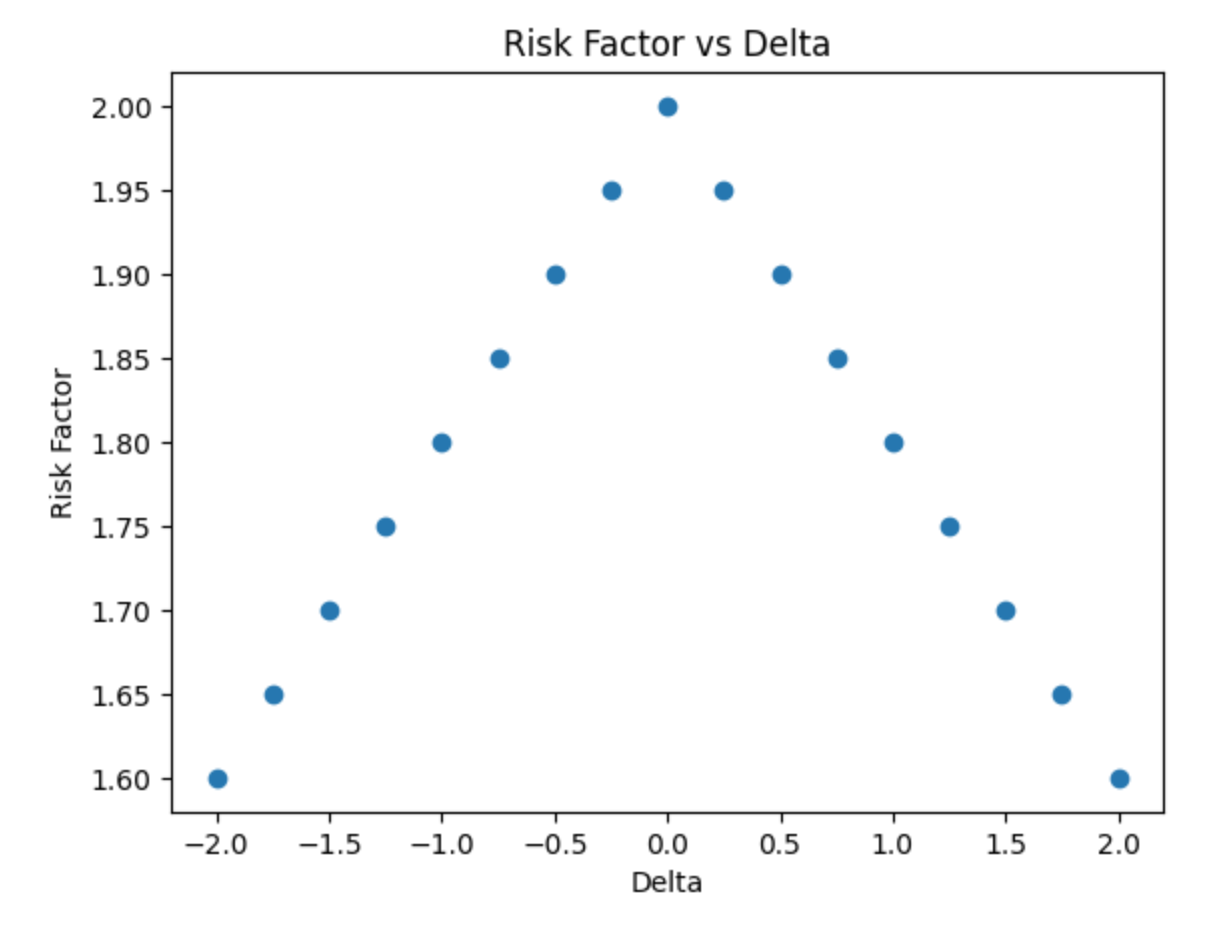
\includegraphics[height=1cm]{images/delta_vs_rf.png}


As we can see, perfectly hedged portfolios achieve the highest Risk Factor values, while any directional exposure, both positive and negative, leads to a substantial decrease in Risk Factor.

\section{Conclusions}
The paper describes the process of calculating maintenance margin requirements using scenario analysis, Reference Price, Liquidation Routing, Mark Price, and Market Impact Factor to manage risk in a cross-chain DeFi ecosystem. The article provides a detailed explanation of these concepts and metrics, including how to estimate the Market Impact Factor for different types of DEXs and perform scenario analysis of constant-product and concentrated liquidity AMMs. 

Further research will include building a more sophisticated Liquidation Routing system, which should be more robust and decrease market impact and slippage.



\bibliographystyle{plain}
\bibliography{references.bib}

\newpage

\begin{appendices}
\end{appendices}


\end{document}